\uuid{eWWl}
\exo7id{5416}
\titre{exo7 5416}
\auteur{rouget}
\organisation{exo7}
\datecreate{2010-07-06}
\isIndication{false}
\isCorrection{true}
\chapitre{Dérivabilité des fonctions réelles}
\sousChapitre{Théorème de Rolle et accroissements finis}
\module{Analyse}
\niveau{L1}
\difficulte{}

\contenu{
\texte{
Soit $f$ une fonction dérivable sur $\Rr$ à valeurs dans $\Rr$ vérifiant $f(0)=f(a)=f'(0)=0$ pour un certain $a$ non nul. Montrer qu'il existe un point distinct de $O$ de la courbe représentative de $f$ en lequel la tangente passe par l'origine.
}
\reponse{
$$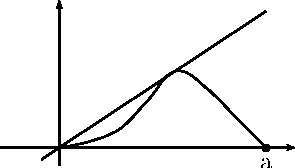
\includegraphics{../images/pdf/eWWl-1.pdf}$$


Soit $x_0$ un réel non nul. Une équation de la tangente $(T_{x_0})$ à la courbe représentative de $f$ au point d'abscisse $x_0$ est $y=f'(x_0)(x-x_0)+f(x_0)$. $(T_{x_0})$ passe par l'origine si et seulement si 

$$x_0f'(x_0)-f(x_0)=0.$$

Pour $x$ réel, on pose $g(x)=\left\{
\begin{array}{l}
\frac{f(x)}{x}\;\mbox{si}\;x\neq0\\
0\;\mbox{si}\;x=0
\end{array}
\right.$ ($g$ est \og~la fonction pente à l'origine~\fg).

Puisque $f$ est continue et dérivable sur $\Rr$, $g$ est déjà continue et dérivable sur $\Rr^*$.

Puisque $f$ est dérivable en $0$ et que $f(0)=f'(0)=0$, $g$ est de plus continue en $0$.

Finalement, $g$ est continue sur $[0,a]$, dérivable sur $]0,a[$ et vérifie $g(0)=g(a)(= 0)$. D'après le théorème de \textsc{Rolle}, il existe un réel $x_0$ dans $]0,a[$ tel que $g'(x_0)=0$. Puisque $x_0$ n'est pas nul, on a $g'(x_0)=\frac{x_0f'(x_0)-f(x_0)}{x_0^2}$. L'égalité $g'(x_0)=0$ s'écrit $x_0f'(x_0)-f(x_0)=0$ et, d'après le début de l'exercice, la tangente à la courbe représentative de $f$ au point d'abscisse $x_0$ passe par l'origine.
}
}
